\begin{enumerate}[label=\thechapter.\arabic*,ref=\thechapter.\theenumi]
    \item The Fourier transform X\brak{j\omega} of the signal\\ $x(t)=\frac{t}{\brak{1+t^2}^2}$ is \rule{1.5cm}{0.15mm}.\hfill{GATE-2022-EC-15}
\begin{enumerate}
	\item[(A)] $\frac{\pi}{2j}\omega e^{-\abs{\omega}}$
	\item[(B)] $\frac{\pi}{2}\omega e^{-\abs{\omega}}$
	\item[(C)] $\frac{\pi}{2j}e^{-\abs{\omega}}$
	\item[(D)] $\frac{\pi}{2}e^{-\abs{\omega}}$
\end{enumerate}

\solution
\iffalse
\let\negmedspace\undefined
\let\negthickspace\undefined
\documentclass[journal,12pt,twocolumn]{IEEEtran}
\usepackage{cite}
\usepackage{amsmath,amssymb,amsfonts,amsthm}
\usepackage{algorithmic}
\usepackage{graphicx}
\usepackage{textcomp}
\usepackage{xcolor}
\usepackage{txfonts}
\usepackage{listings}
\usepackage{enumitem}
\usepackage{mathtools}
\usepackage{gensymb}
\usepackage{comment}
\usepackage[breaklinks=true]{hyperref}
\usepackage{tkz-euclide} 
\usepackage{listings}
\usepackage{gvv}                                        
\def\inputGnumericTable{}                                 
\usepackage[latin1]{inputenc}                                
\usepackage{color}                                            
\usepackage{array}                                            
\usepackage{longtable}                                       
\usepackage{calc}                                             
\usepackage{multirow}                                         
\usepackage{hhline}                                           
\usepackage{ifthen}                                           
\usepackage{lscape}
\usepackage[center]{caption} % center the captions to figure

\newtheorem{theorem}{Theorem}[section]
\newtheorem{problem}{Problem}
\newtheorem{proposition}{Proposition}[section]
\newtheorem{lemma}{Lemma}[section]
\newtheorem{corollary}[theorem]{Corollary}
\newtheorem{example}{Example}[section]
\newtheorem{definition}[problem]{Definition}
\newcommand{\BEQA}{\begin{eqnarray}}
\newcommand{\EEQA}{\end{eqnarray}}
\newcommand{\define}{\stackrel{\triangle}{=}}
\theoremstyle{remark}
\newtheorem{rem}{Remark}
\begin{document}

\newcolumntype{M}[1]{>{\centering\arraybackslash}m{#1}}
\newcolumntype{N}{@{}m{0pt}@{}}

\bibliographystyle{IEEEtran}
\vspace{3cm}

\title{GATE 2022 BM 14 Q} 
\author{ee23btech11223 - Soham Prabhakar More% <-this % stops a space
}
\maketitle
\newpage
\bigskip

\renewcommand{\thefigure}{\theenumi}
\renewcommand{\thetable}{\theenumi}

\bibliographystyle{IEEEtran}

\textbf{Question:} $x\brak{t}$ is a real continuous-time signal whose magnitude frequency response
$\abs{X\brak{j\Omega}}$ is shown below. After sampling $x\brak{t}$ at 100 $rad.s^{-1}$, the spectral point P
is down-converted to \rule{1cm}{0.15mm} $rad.s^{-1}$ in the spectrum of the sampled signal.
\hfill{(GATE 2022 BM 14 Q)}
\begin{figure}[h!]
    \renewcommand\thefigure{1}
    \centering
    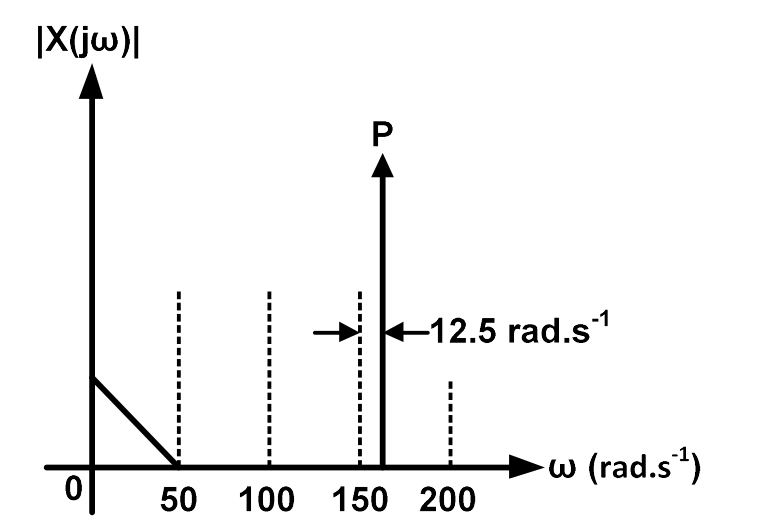
\includegraphics[width=\columnwidth]{2022/BM/14/figs/question.png}
    \caption[short]{Plot of $\abs{X\brak{j\omega}}$}
    \label{fig:2023.bm.14.img1}
\end{figure}

\solution
\fi
\begin{table}[ht]
    \renewcommand\thetable{1}
\begin{tabular}{|c|c|}
    \hline 
    \textbf{Parameter}&\textbf{Description} \\
    \hline
    $w\brak{t}$ & Sampling Function \\
    \hline
	$W\brak{j\omega}$ & Fourier Transform of $w\brak{t}$ \\
    \hline
    $x\brak{t}$ & Input Signal \\
    \hline
    $X\brak{j\omega}$ & Input Signal Frequency Spectrum \\
    \hline
    $x_s\brak{t}$ & Sampled Input Signal \\
    \hline
    $X_s\brak{j\omega}$ & Sampled Signal Frequency Spectrum \\
    \hline
\end{tabular}

\caption{Table of parameters}
\label{Table:1}


\end{table} \\
The sampling function is:
\begin{align}
    w(t) &= \sum_{k = -\infty}^{\infty}\delta\brak{t - \frac{2\pi k}{100}} \\
    W(j\omega) &= 100\sum_{k = -\infty}^{\infty}\delta\brak{j\brak{\omega - 100k}}
\end{align}
then the sampled function: 
\begin{align}
    x_s\brak{t} &= x\brak{t}w\brak{t} \\
    X_s\brak{j\omega} &= X\brak{j\omega} * W\brak{j\omega} \\
    X_s\brak{j\omega} &= \int_{-\infty}^{\infty}X\brak{j\theta}W\brak{j\brak{\omega - \theta}}d\theta \\
    X_s\brak{j\omega} &= 100\sum_{k = -\infty}^{\infty}\int_{-\infty}^{\infty}X\brak{j\theta}\delta\brak{j\brak{\omega - 100k - \theta}}d\theta \\
    X_s\brak{j\omega} &= 100\sum_{k = -\infty}^{\infty}X\brak{j\brak{\omega - 100k}} 
\end{align}
Thus, The down sampled point is at:
\begin{align}
    \omega &= \abs{162.5 - 100k}
\end{align}
where $k$ is the nearest integer to $\frac{162.5}{100}$, which is 2\\
Thus,
\begin{align}
    \omega = 37.5\,rad\,s^{-1}
\end{align}

\begin{figure}[h!]
    \renewcommand\thefigure{2}
    \centering
    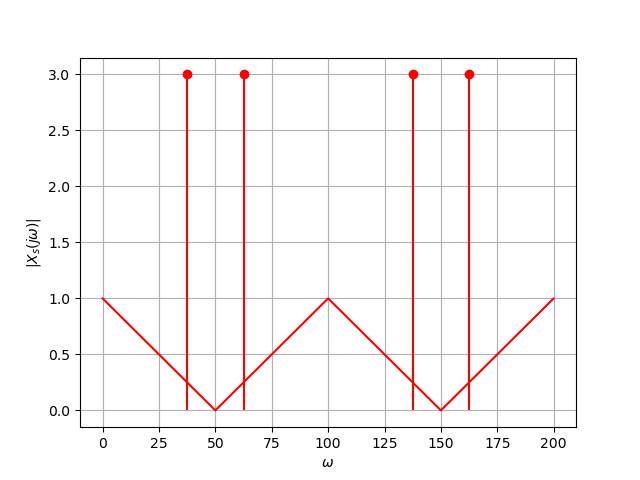
\includegraphics[width=\columnwidth]{2022/BM/14/figs/X_s.png}
    \caption[short]{Plot of $\abs{X_s\brak{j\omega}}$}
    \label{fig:2023.bm.14.img2}
\end{figure}

%\end{document}

\pagebreak

\item For a vector $\bar{x} = [x[0], x[1], \dots, x[7] ]$, the $8$-point discrete Fourier transform (DFT) is denoted by $\bar{X} = \text{DFT}(\bar{x}) = [X[0],X[1],\dots,X[7]]$, where
    \begin{align*}
    X[k] = \sum_{n=0}^{7}x[n]\exp\left(-j\frac{2\pi}{8}nk\right).
    \end{align*} 
    Here $j = \sqrt{-1}$. If $\bar{x} = [1,0,0,0,2,0,0,0]$ and $\bar{y} = \text{DFT}(\text{DFT}(\bar{x}))$, then the value of $y[0]$ is.\hfill{GATE-2022-EC-55}\\
    \solution
    \input{2022/EC/55/55.tex}
    \pagebreak
\item \textbf{Question:} An LTI system is shown in the figure where $$H\brak{s}= \frac{100}{s^2+0.1s+10}$$ The steady state output of the system for an input $x\brak{t}$ is given by $y\brak{t}=a+b\sin{\brak{10t+\theta}}$. The values of $'a'$ and $'b'$ are \\\\
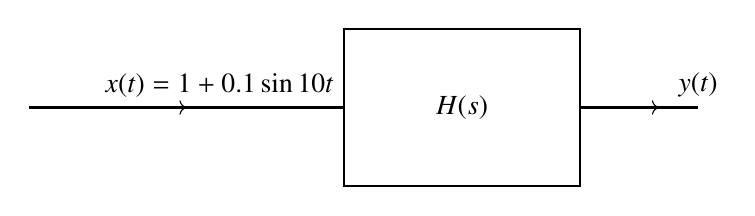
\begin{tikzpicture}
    \draw [thick, draw=black] (-2,-1) -- (2,-1) node[anchor=south east] {$x(t)=1+0.1\sin{\brak{10t}}$};
    \draw [thick,draw=black] (2,0) rectangle (5,-2) ;
    \draw [thick,draw=black] (5,-1) -- (6.5,-1) node[anchor=south] {$y(t)$};
    \draw [->] (-2,-1)--(0,-1);
    \draw [->] (5,-1)--(6,-1);
    \draw (3.5, -1) node[] {$H(s)$};
\end{tikzpicture}\\
\solution 
    \iffalse
\let\negmedspace\undefined
\let\negthickspace\undefined
\documentclass[journal,12pt,twocolumn]{IEEEtran}
\usepackage{cite}
\usepackage{amsmath,amssymb,amsfonts,amsthm}
\usepackage{algorithmic}
\usepackage{graphicx}
\usepackage{textcomp}
\usepackage{xcolor}
\usepackage{txfonts}
\usepackage{listings}
\usepackage{enumitem}
\usepackage{mathtools}
\usepackage{gensymb}
\usepackage{comment}
\usepackage[breaklinks=true]{hyperref}
\usepackage{tkz-euclide} 
\usepackage{listings}
\usepackage{gvv}                                        
\def\inputGnumericTable{}                                 
\usepackage[latin1]{inputenc}                                
\usepackage{color}                                            
\usepackage{array}                                            
\usepackage{longtable}                                       
\usepackage{calc}                                             
\usepackage{multirow}                                         
\usepackage{hhline}                                           
\usepackage{ifthen}                                           
\usepackage{lscape}
\usepackage[center]{caption} % center the captions to figure

\newtheorem{theorem}{Theorem}[section]
\newtheorem{problem}{Problem}
\newtheorem{proposition}{Proposition}[section]
\newtheorem{lemma}{Lemma}[section]
\newtheorem{corollary}[theorem]{Corollary}
\newtheorem{example}{Example}[section]
\newtheorem{definition}[problem]{Definition}
\newcommand{\BEQA}{\begin{eqnarray}}
\newcommand{\EEQA}{\end{eqnarray}}
\newcommand{\define}{\stackrel{\triangle}{=}}
\theoremstyle{remark}
\newtheorem{rem}{Remark}
\begin{document}

\newcolumntype{M}[1]{>{\centering\arraybackslash}m{#1}}
\newcolumntype{N}{@{}m{0pt}@{}}

\bibliographystyle{IEEEtran}
\vspace{3cm}

\title{GATE 2022 BM 14 Q} 
\author{ee23btech11223 - Soham Prabhakar More% <-this % stops a space
}
\maketitle
\newpage
\bigskip

\renewcommand{\thefigure}{\theenumi}
\renewcommand{\thetable}{\theenumi}

\bibliographystyle{IEEEtran}

\textbf{Question:} $x\brak{t}$ is a real continuous-time signal whose magnitude frequency response
$\abs{X\brak{j\Omega}}$ is shown below. After sampling $x\brak{t}$ at 100 $rad.s^{-1}$, the spectral point P
is down-converted to \rule{1cm}{0.15mm} $rad.s^{-1}$ in the spectrum of the sampled signal.
\hfill{(GATE 2022 BM 14 Q)}
\begin{figure}[h!]
    \renewcommand\thefigure{1}
    \centering
    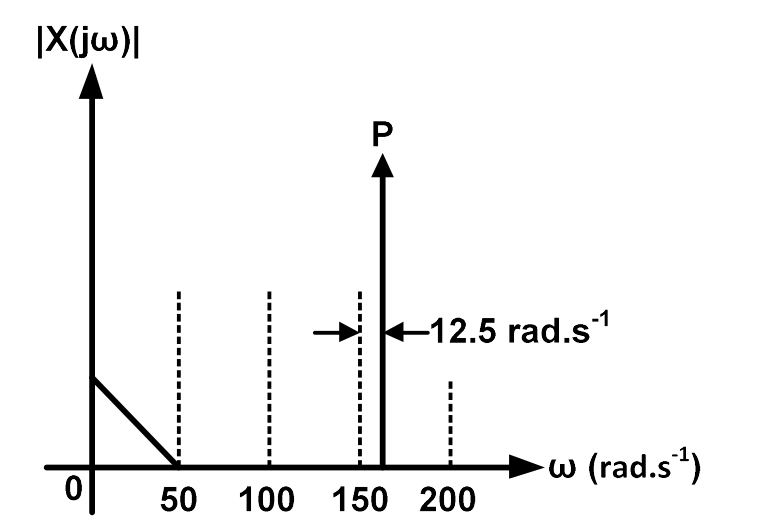
\includegraphics[width=\columnwidth]{2022/BM/14/figs/question.png}
    \caption[short]{Plot of $\abs{X\brak{j\omega}}$}
    \label{fig:2023.bm.14.img1}
\end{figure}

\solution
\fi
\begin{table}[ht]
    \renewcommand\thetable{1}
\begin{tabular}{|c|c|}
    \hline 
    \textbf{Parameter}&\textbf{Description} \\
    \hline
    $w\brak{t}$ & Sampling Function \\
    \hline
	$W\brak{j\omega}$ & Fourier Transform of $w\brak{t}$ \\
    \hline
    $x\brak{t}$ & Input Signal \\
    \hline
    $X\brak{j\omega}$ & Input Signal Frequency Spectrum \\
    \hline
    $x_s\brak{t}$ & Sampled Input Signal \\
    \hline
    $X_s\brak{j\omega}$ & Sampled Signal Frequency Spectrum \\
    \hline
\end{tabular}

\caption{Table of parameters}
\label{Table:1}


\end{table} \\
The sampling function is:
\begin{align}
    w(t) &= \sum_{k = -\infty}^{\infty}\delta\brak{t - \frac{2\pi k}{100}} \\
    W(j\omega) &= 100\sum_{k = -\infty}^{\infty}\delta\brak{j\brak{\omega - 100k}}
\end{align}
then the sampled function: 
\begin{align}
    x_s\brak{t} &= x\brak{t}w\brak{t} \\
    X_s\brak{j\omega} &= X\brak{j\omega} * W\brak{j\omega} \\
    X_s\brak{j\omega} &= \int_{-\infty}^{\infty}X\brak{j\theta}W\brak{j\brak{\omega - \theta}}d\theta \\
    X_s\brak{j\omega} &= 100\sum_{k = -\infty}^{\infty}\int_{-\infty}^{\infty}X\brak{j\theta}\delta\brak{j\brak{\omega - 100k - \theta}}d\theta \\
    X_s\brak{j\omega} &= 100\sum_{k = -\infty}^{\infty}X\brak{j\brak{\omega - 100k}} 
\end{align}
Thus, The down sampled point is at:
\begin{align}
    \omega &= \abs{162.5 - 100k}
\end{align}
where $k$ is the nearest integer to $\frac{162.5}{100}$, which is 2\\
Thus,
\begin{align}
    \omega = 37.5\,rad\,s^{-1}
\end{align}

\begin{figure}[h!]
    \renewcommand\thefigure{2}
    \centering
    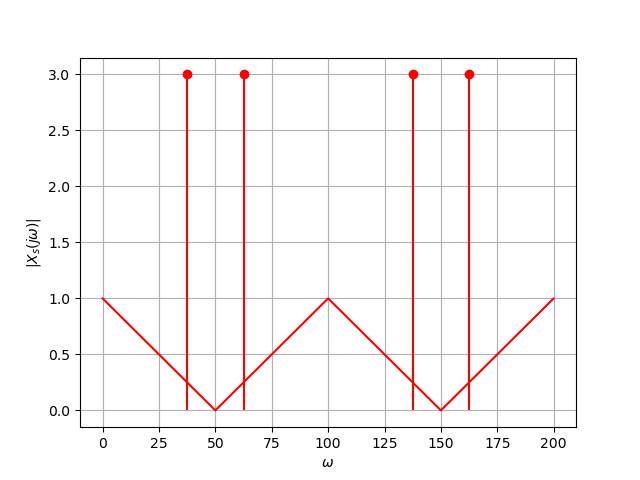
\includegraphics[width=\columnwidth]{2022/BM/14/figs/X_s.png}
    \caption[short]{Plot of $\abs{X_s\brak{j\omega}}$}
    \label{fig:2023.bm.14.img2}
\end{figure}

%\end{document}

\item Consider an ideal full-bridge single-phase DC-AC inverter with a DC bus voltage magnitude of $1000 V$. The inverter output voltage $v(t)$ shown below is obtained when diagonal switches of the inverter are switched with $50\%$ duty cycle. The inverter feeds a load with a sinusoidal current given by $i(t) = 10 \sin(\omega t - \frac{\pi}{3}) \, \mathrm{A}$, where $\omega=\frac{2\pi}{T}$. The active power, in watts, delivered to the load is \underline{\quad}.[Gate2022-EE-58]  \\     
\begin{figure}[htb]
  \centering
  \begin{tikzpicture}
  \begin{axis}[
    xlabel={$t$},
    ylabel={$v(t)$},
    axis lines=middle,
    ymin=-1.5, ymax=1.5,
    xtick={0,0.5,1.0,1.5},
    xticklabels={0, $0.5 T$, $1.0 T$, $1.5 T$},
    ytick={0},
    grid=none,
    enlargelimits=0.2,
    xticklabel style={xshift=-0.4cm},
    height=6cm,
    ]
    \addplot[const plot, thick, blue] coordinates {(0,1) (0.5,1) (0.5,-1) (1,-1) (1,1) (1.5,1)};
  \end{axis}
\end{tikzpicture}




  \label{fig:EE_58_f1}
\end{figure}
\solution
\iffalse
\documentclass[journal,12pt,onecolumn]{IEEEtran}
\usepackage{cite}
\usepackage{amsmath,amssymb,amsfonts,amsthm}
\usepackage{algorithmic}
\usepackage{graphicx}
\usepackage{textcomp}
\usepackage{xcolor}
\usepackage{txfonts}
\usepackage{listings}
\usepackage{enumitem}
\usepackage{mathtools}
\usepackage{gensymb}
\usepackage{comment}
\usepackage[breaklinks=true]{hyperref}
\usepackage{tkz-euclide} 
\usepackage{listings}
\def\inputGnumericTable{}                                 
\usepackage[latin1]{inputenc}                                
\usepackage{color}                                            
\usepackage{array}                                            
\usepackage{longtable}                                       
\usepackage{calc}                                             
\usepackage{multirow}                                         
\usepackage{hhline}                                           
\usepackage{ifthen}                                           
\usepackage{lscape}
\usepackage{caption}
\usepackage{subfigure}
\usepackage{gvv}
\usepackage{pgfplots}
\usepackage{circuitikz}
\usepackage{graphicx}

% Define \phase command
\newcommand{\phase}[1]{\text{arg}\left(#1\right)}

\newtheorem{theorem}{Theorem}[section]
\newtheorem{problem}{Problem}
\newtheorem{proposition}{Proposition}[section]
\newtheorem{lemma}{Lemma}[section]
\newtheorem{corollary}[theorem]{Corollary}
\newtheorem{example}{Example}[section]
\newtheorem{definition}[problem]{Definition}
\newcommand{\BEQA}{\begin{eqnarray}}
\newcommand{\EEQA}{\end{eqnarray}}
\newcommand{\system}[1]{\stackrel{#1}{\rightarrow}}
\newcommand{\define}{\stackrel{\triangle}{=}}
\theoremstyle{remark}
\newtheorem{rem}{Remark}

\begin{document}

\bibliographystyle{IEEEtran}
\vspace{3cm}

\title{Gate-2022-EE-58}
\author{EE22BTECH11008 - Annapureddy Siva Meenakshi$^{*}$}
\maketitle
\bigskip

\renewcommand{\thefigure}{\theenumi}
\renewcommand{\thetable}{\theenumi}
Q: Consider an ideal full-bridge single-phase DC-AC inverter with a DC bus voltage magnitude of $1000 V$. The inverter output voltage $v(t)$ shown below is obtained when diagonal switches of the inverter are switched with $50\%$ duty cycle. The inverter feeds a load with a sinusoidal current given by $i(t) = 10 \sin(\omega t - \frac{\pi}{3}) \, \mathrm{A}$, where $\omega=\frac{2\pi}{T}$. The active power, in watts, delivered to the load is \underline{\quad}.[Gate2022-EE-58]  \\     
\begin{figure}[htb]
  \centering
  \begin{tikzpicture}
  \begin{axis}[
    xlabel={$t$},
    ylabel={$v(t)$},
    axis lines=middle,
    ymin=-1.5, ymax=1.5,
    xtick={0,0.5,1.0,1.5},
    xticklabels={0, $0.5 T$, $1.0 T$, $1.5 T$},
    ytick={0},
    grid=none,
    enlargelimits=0.2,
    xticklabel style={xshift=-0.4cm},
    height=6cm,
    ]
    \addplot[const plot, thick, blue] coordinates {(0,1) (0.5,1) (0.5,-1) (1,-1) (1,1) (1.5,1)};
  \end{axis}
\end{tikzpicture}




  \label{fig:EE_58_f1}
\end{figure}
   
\fi
\solution

\begin{table}[!ht]
    \centering
        \begin{tabular}{|c|c|c|} 
    \hline
    \textbf{Variable} & \textbf{Description} & \textbf{Value} \\
    \hline
    $V_\text{s}$ & input DC voltage & $1000V$ \\
    \hline
    $i(t)$ & output current & $\sin(\omega t-\frac{\pi}{3})$ \\
    \hline
    $v(t)$ & Output voltage & given \\
    \hline 
    $\omega$& Frequency &  $\frac{2\pi}{T}$     \\
    \hline
       $v_{0}^{\text{rms}}$&  RMS output voltage at the fundamental frequency& none\\
    \hline
    $i_{\text{rms}}$&  RMS output current at the fundamental frequency& none\\
    \hline
     $v_{0}(t)$&  output voltage at the fundamental frequency& none\\
    \hline
    $\phi$ & phase difference between $v_{0}(t)$ and $i(t)$&none\\
    \hline
    $i_{0}$& amplitude of output current & $1$\\
    \hline
    $P$&        active power delivered&none\\
    \hline
\end{tabular}

    \caption{Input parameters}
    \label{tab:EE_58_t1}
\end{table}

\begin{figure}[htb]
  \centering
  \begin{tikzpicture}

% Draw rectangle for inverter
\draw (0,0) rectangle (2,2);
\node at (1,1) {DC-AC};

% Draw input lines with battery
\draw (-1,1.5) -- (0,1.5) node[midway, left] {};
\draw (-1,0.5) -- (0,0.5) node[midway, left] {};

% Draw output lines
\draw (2,1.5) -- (3,1.5) node[right] {};
\draw (2,0.5) -- (3,0.5) node[right] {};

% Draw load resistor symbol with rotated text
\draw (2.9,0.7) rectangle (3.1,1.3) node[midway, rotate=90] {\rotatebox{-180}{\tiny Load}};

\draw (3,1.3) -- (3,1.5) node[right] {};
\draw (3,0.5) -- (3,0.7) node[right] {};

% Draw battery symbol without arrow and label
\draw (-1,1.5) to [battery1] (-1,0.5);
\node at (-2.1,1) {\tiny $V_\text{s}=1000V DC$};

% Draw current arrow
\draw[->] (3,1.5) -- (3,1.3) node[midway, above] {};

% Add labels for the current arrow
\node at (4.1,1.4) {\tiny $i(t)=\sin(\omega t-\frac{\pi}{3})$};
\node at (2.2,1.4) {\tiny $+$};
\node at (2.2,1) {\tiny $V_0$};
\node at (2.2,0.6) {\tiny $-$};
\end{tikzpicture}


   \captionsetup{justification=centering, singlelinecheck=off}
  \caption{circuit diagram of the system}
  \label{fig:EE_58_f2}
\end{figure}

The Fourier series expansion of the given voltage $v(t)$ is,
\begin{align}
  v(t) &= \sum_{n=1,3,5,\ldots}^{\infty} \frac{4V_{\text{dc}}}{n\pi} \sin(n\omega t)\\
    v_{0}(t)&=  \frac{4V_{\text{dc}}}{\pi} \sin(\omega t)\\
    \therefore \quad \phi &= \frac{\pi}{3}\\
    v_{0}^{\text{rms}}&=  \frac{4V_{\text{dc}}}{\pi \sqrt{2}}\\
    &=\frac{4000}{\pi \sqrt{2}}\\
    i_{\text{rms}}&=\frac{i_{0}}{\sqrt{2}}=\frac{1}{\sqrt{2}}
\end{align}
  Active power delivered to load in Watts is given by,
  \begin{align}
    P &= v_{0}^{\text{rms}} \times i_{\text{rms}} \times \cos{\phi}\\
    &= \frac{4000}{\pi \sqrt{2}} \times \frac{1}{\sqrt{2}} \times \cos{\frac{\pi}{3}}\\
    &\approx 3183 
\end{align}

\begin{figure}[htb]
  \centering
  \begin{tikzpicture}
  \begin{axis}[
    xlabel={$t$},
    ylabel={$v(t)$},
    axis lines=middle,
    ymin=-1.5, ymax=1.5,
    xtick={0,0.5,1.0,1.5},
    xticklabels={0, $0.5 T$, $1.0 T$, $1.5 T$},
    ytick={0},
    grid=none,
    enlargelimits=0.2,
    xticklabel style={xshift=-0.4cm},
    height=6cm,
    ]
    \addplot[const plot, thick, blue] coordinates {(0,1) (0.5,1) (0.5,-1) (1,-1) (1,1) (1.5,1)};
  \end{axis}
\end{tikzpicture}




   \captionsetup{justification=centering, singlelinecheck=off}
  \caption{output voltage and current of the system}
  \label{fig:EE_58_f3}
\end{figure}

%\end{document}


\pagebreak
\end{enumerate}
